\renewcommand{\thesubfigure}{\alph{subfigure}}
\section{Evaluation}
\subsection{Setup}
To comprehensively evaluate the quality of instruction-tuned models, we employ a diverse suite of benchmarks categorized into five dimensions:

\begin{itemize}
    \item \textbf{Knowledge}: MMLU \citep{hendrycks2020mmlu}, MMLU-Pro \citep{wang2024mmlupro}, GPQA-Diamond \citep{rein2024gpqa}, ARC \citep{clark2018think}, CMMLU \citep{li2023cmmlu} C-Eval \citep{huang2023ceval}, GAOKAO-Bench \citep{zhang2023evaluating}, SciBench \citep{wang2023scibench}, PHYBench \citep{qiu2025phybench}, TriviaQA \citep{joshi2017triviaqa}
    \item \textbf{Reasoning}: SQuAD 2.0 \citep{rajpurkar2018know}, DROP \citep{dua2019drop}, KOR-Bench \citep{ma2024kor}, HellaSwag \citep{zellers2019hellaswag}, BIG-Bench Hard \citep{suzgun2023challenging}, BIG-Bench Extra Hard \citep{kazemi2025big}, MuSR \citep{sprague2023musr}, ZebraLogic \citep{lin2025zebralogic}, PrOntoQA \citep{saparov2022language}, PIQA \citep{bisk2020piqa}, OCNLI \citep{hu2020ocnli}, BIG-Bench Hard-CN \citep{opencompass}
    \item \textbf{Coding}: CRUXEval \citep{gu2024cruxeval}, MBPP \citep{austin2021program}, MultiPL-E \citep{cassano2023multiple}, HumanEval \citep{chen2021evaluating}, BigCodeBench \citep{zhuo2024bigcodebench}, LiveCodeBench \citep{jain2024livecodebench}, Spider \citep{yu2018spider}, BIRD \citep{li2023can}, HumanEval+ \citep{liu2023your}, MBPP+ \citep{liu2023your}, HumanEvalFix \citep{muennighoff2023octopack}, Aider \citep{aider}, HumanEval-CN \citep{opencompass}
    \item \textbf{Math}: GSM8K \citep{cobbe2021gsm8k}, MATH \citep{hendrycks2021math}, OlympiadBench \citep{he2024olympiadbench}, AIME 2025 \citep{aime2025aime}, Omni-MATH \citep{gao2024omni}, HARDMath2 \citep{roggeveen2025hardmath2}, GSM-Plus \citep{li2024gsm}, CMATH \citep{wei2023cmath}
    \item \textbf{Agent \& Alignment}: BFCL \citep{patil2025bfcl}, IFEval \citep{zhou2023ifeval}, CodeIF-Bench \citep{wang2025codeif}, Nexus Function Calling Benchmark \citep{nexusraven}
\end{itemize}

This extensive evaluation suite, comprising a total of 47 benchmarks, provides a holistic foundation for assessing model capabilities. In our experiments, we compare the LLaDA2.0 series against strong open-source auto-regressive (AR) models.

For all LLaDA2.0 models, we utilize a temperature of 0.0, a block size of 32, and a decoding threshold of 0.95.

\subsection{Results}
The overall results, presented in the following tables, indicate that the LLaDA2.0 architecture is not only highly competitive, but also shows a promising trend of closing the performance gap with, and even surpassing, AR models in specific key areas. Our models consistently demonstrate strong, and often superior, performance in complex, structured tasks. For instance, LLaDA2.0-mini already outperforms a comparable AR model (Qwen3-8B) in the domains of Reasoning, Coding, and Math. This signal is amplified in our larger model, as LLaDA2.0-flash achieves parity with the powerful Qwen3-30B-A3B-Instruct-2507 and establishes a lead in the critical Coding and Agent domains. This suggests that as diffusion models scale, their inherent strengths in structured generation and tool use become increasingly apparent.

\begin{table}[htbp]
\centering
\caption{Benchmark Performance of LLaDA2.0-mini}
\label{tab:mini_benchmark}
% 如果表格太宽，可以使用 \resizebox 来缩放到页面宽度
\resizebox{\textwidth}{!}{%
\begin{tabular}{lcccc}
\toprule
\textbf{Benchmark} & \textbf{Qwen3-8B (no\_think)} & \textbf{Ling-mini-2.0} & \textbf{LLaDA2.0-mini-preview} & \textbf{LLaDA2.0-mini} \\
\midrule
\textbf{Average} & 63.42 & 65.77 & 54.67 & 64.34 \\
\midrule
\multicolumn{5}{c}{\textbf{Knowledge}} \\
\midrule
MMLU & 80.94 & 82.15 & 72.49 & 80.53 \\
MMLU-Pro & 65.48 & 63.72 & 49.22 & 63.22 \\
CMMLU & 79.17 & 80.84 & 67.53 & 79.50 \\
C-EVAL & 81.36 & 82.10 & 66.54 & 81.38 \\
GAOKAO-Bench & 84.94 & 87.23 & 74.46 & 84.30 \\
ARC-c & 93.35 & 93.09 & 89.15 & 93.56 \\
GPQA & 46.59 & 56.80 & 23.74 & 47.98 \\
SciBench & 2.85 & 5.28 & 4.10 & 3.53 \\
PHYBench & 9.76 & 14.59 & 5.08 & 11.70 \\
TriviaQA & 52.51 & 55.63 & 50.49 & 51.33 \\
\midrule
\multicolumn{5}{c}{\textbf{Reasoning}} \\
\midrule
BIG-Bench Hard & 79.48 & 83.70 & 70.64 & 78.21 \\
BIG-Bench Extra Hard & 18.27 & 14.81 & 12.36 & 16.47 \\
bbh-zh & 80.09 & 66.11 & 66.62 & 75.75 \\
MuSR & 70.02 & 71.36 & 56.77 & 71.48 \\
ZebraLogic & 37.48 & 79.85 & 14.80 & 64.20 \\
PrOntoQA & 93.12 & 96.06 & 70.00 & 86.00 \\
PIQA & 88.30 & 87.54 & 84.33 & 86.51 \\
OCNLI & 61.49 & 60.17 & 58.68 & 64.51 \\
HellaSwag & 79.56 & 69.02 & 74.01 & 79.01 \\
KOR-Bench & 54.48 & 62.72 & 37.26 & 50.40 \\
DROP & 84.56 & 78.80 & 79.49 & 81.91 \\
SQuAD 2.0 & 85.21 & 75.56 & 85.61 & 86.50 \\
\midrule
\multicolumn{5}{c}{\textbf{Coding}} \\
\midrule
CRUXEval-O & 74.06 & 76.12 & 61.88 & 71.62 \\
MBPP & 78.92 & 84.07 & 77.75 & 81.50 \\
MBPP+ & 71.96 & 76.46 & 66.67 & 74.07 \\
MultiPL-E & 61.70 & 67.09 & 62.43 & 67.46 \\
HumanEval & 84.76 & 85.98 & 80.49 & 86.59 \\
HumanEval+ & 78.66 & 81.71 & 71.95 & 79.88 \\
HumanEvalFix & 76.02 & 82.83 & 60.16 & 74.90 \\
HumanEval-cn & 74.39 & 71.34 & 73.17 & 78.66 \\
BigCodeBench-Full & 36.05 & 35.00 & 30.44 & 32.89 \\
LiveCodeBench & 26.38 & 34.97 & 19.82 & 31.50 \\
Aider & 55.64 & 49.62 & 28.57 & 39.85 \\
BIRD-SQL & 36.11 & 39.67 & 27.71 & 39.34 \\
Spider & 72.80 & 76.43 & 75.64 & 76.76 \\
\midrule
\multicolumn{5}{c}{\textbf{Math}} \\
\midrule
GSM8K & 93.63 & 94.62 & 89.01 & 94.24 \\
MATH & 86.28 & 94.66 & 73.50 & 93.22 \\
OlympiadBench & 55.33 & 72.30 & 36.30 & 67.70 \\
AIME 2025 & 22.08 & 47.66 & 10.00 & 36.67 \\
HARDMath2 & 7.58 & 9.95 & 0.95 & 0.47 \\
Omni-MATH & 33.20 & 48.80 & 19.20 & 41.70 \\
GSM-Plus & 86.09 & 87.82 & 81.44 & 86.24 \\
CMATH & 95.42 & 96.40 & 90.53 & 95.72 \\
\midrule
\multicolumn{5}{c}{\textbf{Agent \& Alignment}} \\
\midrule
IFEval-strict-prompt & 86.90 & 76.16 & 62.50 & 80.78 \\
BFCL v3 & 70.08 & 53.98 & 74.11 & 70.90 \\
CodeIF-Bench & 50.00 & 46.00 & 48.00 & 48.00 \\
Nexus FC & 37.71 & 34.38 & 33.68 & 35.18 \\
\bottomrule
\end{tabular}%
} % 如果使用了 \resizebox，在这里结束
\end{table}
\begin{table}[htbp]
\centering
\caption{Benchmark Performance of LLaDA2.0-flash}
\label{tab:flash_benchmark}
% 由于表头较长，建议取消下面两行注释以缩放表格适应页面宽度
\resizebox{\textwidth}{!}{%
\begin{tabular}{lcccc}
\toprule
\textbf{Benchmark} & \textbf{Qwen3-30B-A3B-Instruct-2507} & \textbf{Ling-flash-2.0} & \textbf{LLaDA2.0-flash-preview} & \textbf{LLaDA2.0-flash} \\
\midrule
\textbf{Average} & 73.60 & 72.15 & 65.97 & 73.18 \\
\midrule
\multicolumn{5}{c}{\textbf{Knowledge}} \\
\midrule
MMLU & 87.13 & 87.98 & 83.15 & 87.69 \\
MMLU-Pro & 74.23 & 76.84 & 66.16 & 73.36 \\
CMMLU & 86.36 & 86.59 & 79.64 & 85.13 \\
C-EVAL & 88.17 & 88.03 & 79.28 & 86.75 \\
GAOKAO-Bench & 94.53 & 93.24 & 86.12 & 93.90 \\
ARC-c & 95.81 & 95.08 & 93.90 & 95.93 \\
GPQA & 57.34 & 67.12 & 41.92 & 61.98 \\
SciBench & 4.54 & 4.14 & 5.13 & 4.13 \\
PHYBench & 29.84 & 27.67 & 7.58 & 30.06 \\
TriviaQA & 65.61 & 69.76 & 69.25 & 66.88 \\
\midrule
\multicolumn{5}{c}{\textbf{Reasoning}} \\
\midrule
BIG-Bench Hard & 85.54 & 89.36 & 82.85 & 86.75 \\
BIG-Bench Extra Hard & 37.80 & 23.24 & 16.70 & 27.86 \\
BIG-Bench Hard - CN & 86.18 & 75.09 & 83.38 & 87.52 \\
MuSR & 79.15 & 82.72 & 78.75 & 80.48 \\
ZebraLogic & 90.97 & 87.60 & 39.90 & 82.30 \\
PrOntoQA & 97.12 & 97.88 & 93.50 & 96.50 \\
PIQA & 91.57 & 91.95 & 91.84 & 92.76 \\
OCNLI & 71.59 & 65.36 & 69.39 & 71.63 \\
HellaSwag & 86.31 & 81.59 & 86.00 & 84.97 \\
KOR-Bench & 68.00 & 68.96 & 53.28 & 64.24 \\
DROP & 87.57 & 88.32 & 88.17 & 87.90 \\
SQuAD 2.0 & 89.51 & 81.32 & 90.61 & 90.00 \\
\midrule
\multicolumn{5}{c}{\textbf{Coding}} \\
\midrule
CRUXEval-O & 86.75 & 82.75 & 74.50 & 85.12 \\
MBPP & 86.65 & 85.01 & 86.65 & 88.29 \\
MBPP+ & 78.04 & 76.19 & 75.93 & 79.63 \\
MultiPL-E & 70.67 & 65.76 & 72.38 & 74.87 \\
HumanEval & 93.29 & 85.98 & 88.41 & 94.51 \\
HumanEval+ & 88.41 & 85.98 & 82.32 & 87.80 \\
HumanEvalFix & 91.16 & 92.68 & 83.33 & 90.24 \\
HumanEval-CN & 87.20 & 74.39 & 84.76 & 89.02 \\
Bigcodebench-Full & 41.49 & 40.70 & 40.44 & 41.58 \\
LiveCodeBench & 41.63 & 44.11 & 29.07 & 42.29 \\
Aider & 71.43 & 71.43 & 51.13 & 66.92 \\
Spider & 81.79 & 80.58 & 81.37 & 82.49 \\
BIRD-SQL & 47.75 & 47.49 & 45.34 & 45.76 \\
\midrule
\multicolumn{5}{c}{\textbf{Math}} \\
\midrule
GSM8K & 96.36 & 95.45 & 95.75 & 96.06 \\
MATH & 96.70 & 96.10 & 83.52 & 95.44 \\
OlympiadBench & 77.59 & 76.19 & 49.33 & 74.07 \\
AIME 2025 & 61.88 & 55.89 & 23.33 & 60.00 \\
HARDMath2 & 4.27 & 23.70 & 3.79 & 4.27 \\
Omni-MATH & 54.00 & 53.00 & 24.60 & 50.30 \\
GSM-Plus & 89.45 & 89.83 & 88.25 & 89.64 \\
CMATH & 96.58 & 96.52 & 95.26 & 96.90 \\
\midrule
\multicolumn{5}{c}{\textbf{Agent \& Alignment}} \\
\midrule
IFEval-strict -prompt & 84.29 & 81.52 & 75.60 & 81.70 \\
BFCL v3 & 73.19 & 67.57 & 74.86 & 75.43 \\
CodeIF-Bench & 54.00 & 56.00 & 56.00 & 58.00 \\
Nexus FC & 49.93 & 36.25 & 47.98 & 50.45 \\
\bottomrule
\end{tabular}%
} % 如果使用了 \resizebox，在这里结束
\end{table}

As shown in \Cref{tab:mini_benchmark}, \textbf{LLaDA2.0-mini} achieves a competitive average score of 64.34, closely approaching its AR peer, Ling-mini-2.0 (65.77). This demonstrates the fundamental viability of the diffusion approach. More importantly, it shows promising signals in complex tasks, outperforming its direct competitor on reasoning benchmarks like SQuAD 2.0 (86.50) and demonstrating more robust instruction following on IFEval (80.78). Its strong performance in coding tasks such as HumanEval (86.59) further suggests an early aptitude for structured generation.

This potential becomes even more evident with our larger model, \textbf{LLaDA2.0-flash}. As shown in \Cref{tab:flash_benchmark}, with an average score of 73.18, it stands firmly on par with strong AR models such as Qwen3-30B-A3B-Instruct-2507 (73.60). Crucially, LLaDA2.0-flash begins to exhibit clear advantages in complex generative tasks, a sign that the diffusion architecture may hold inherent strengths. In the critical domain of coding, it consistently outperforms its AR peers, scoring higher on HumanEval (94.51), MBPP (88.29) and MultiPL-E (74.87). This trend of surpassing AR models also extends to agent capabilities (BFCL v3: 75.43) and advanced mathematics (AIME 2025: 60.00).

In conclusion, the LLaDA2.0 series successfully demonstrates that diffusion-based language models are a powerful and scalable alternative to the dominant auto-regressive paradigm. While rapidly narrowing the gap on general benchmarks, they are already showcasing the potential to surpass traditional architectures in complex, structured domains like code generation and tool use. This positions diffusion models as a highly promising direction for the future of language generation.

\subsection{Analysis}
\paragraph{Analysis of Inference Hyper-parameters}

In addition to our main evaluation, we conducted a brief analysis to tune key inference hyperparameters. To ensure efficiency, this analysis was performed on our LLaDA2.0-mini model, using a representative subset of our benchmarks to understand the trade-off between generation quality (score) and inference speed (measured as TPF - Tokens Per Forward; higher is faster).

\begin{figure}[t]
    \centering
    \small
    \begin{minipage}{0.47\textwidth}
        \centering
        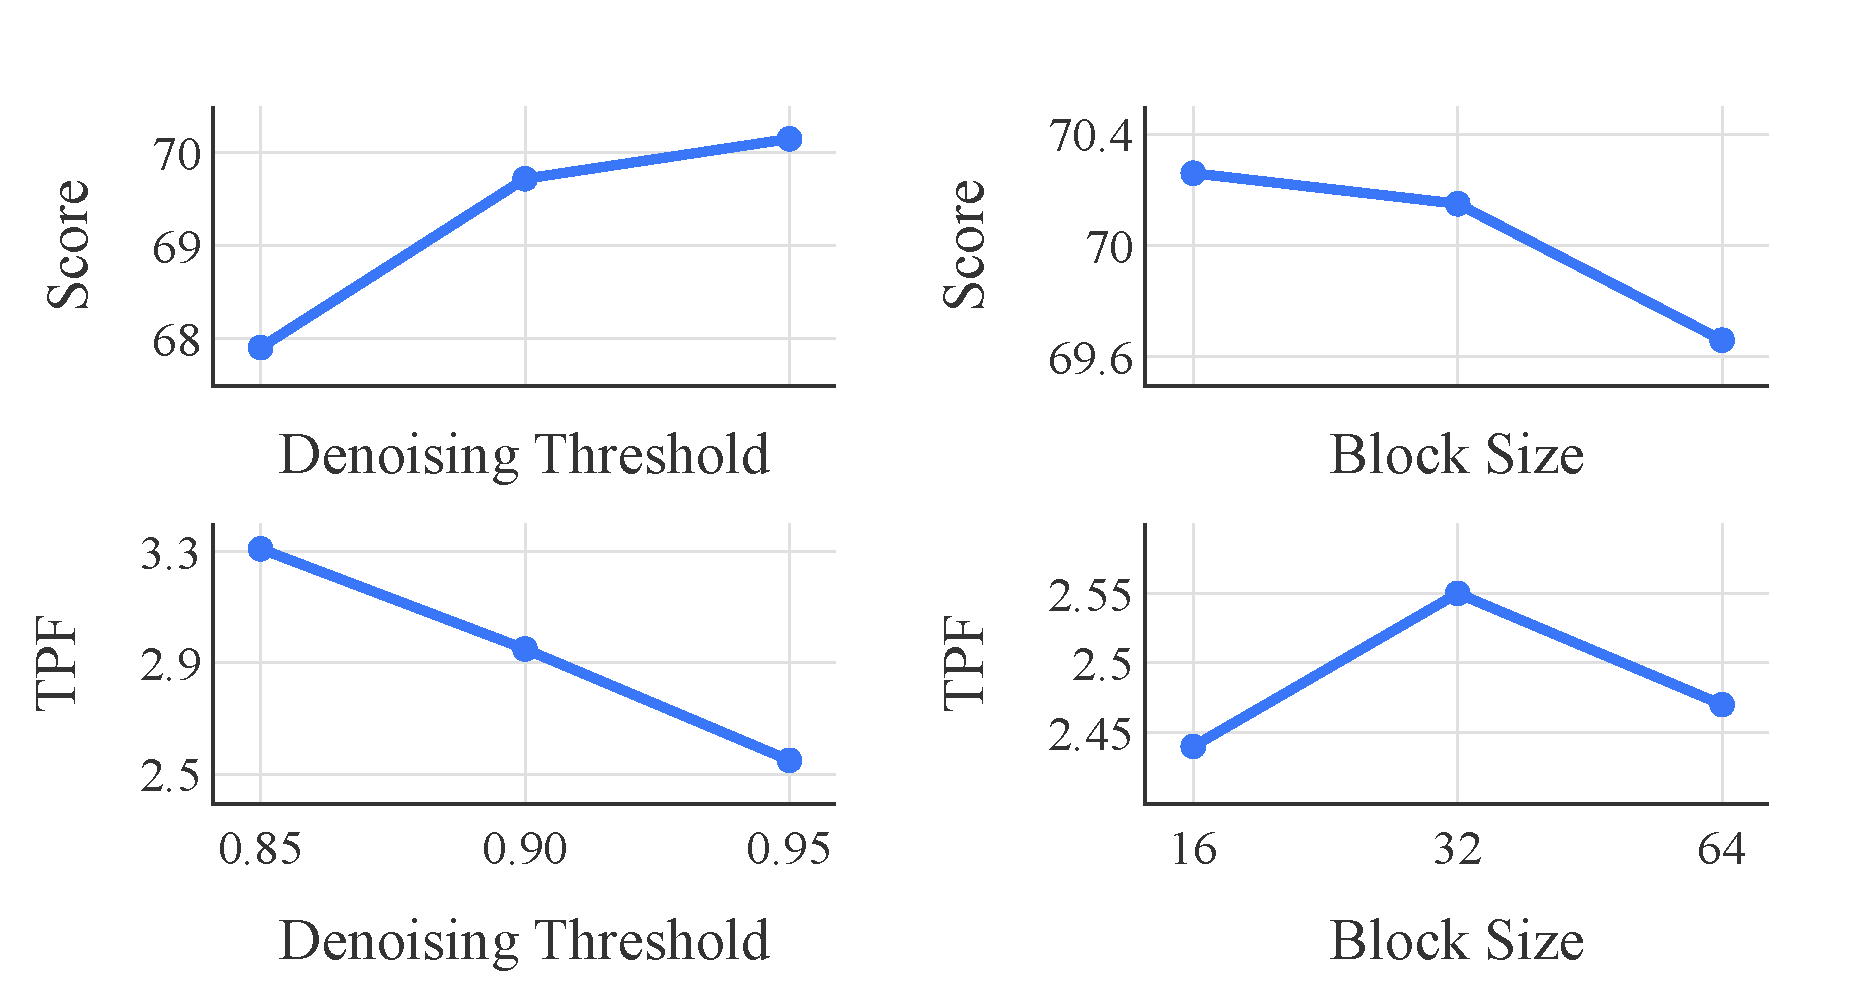
\includegraphics[width=\linewidth]{images/llada2_line_tps_score}
        \caption{Score/TPF vs threshold/block size}
        \label{fig:params}
    \end{minipage}%
    \hfill
    \begin{minipage}{0.5\textwidth}
        \centering
        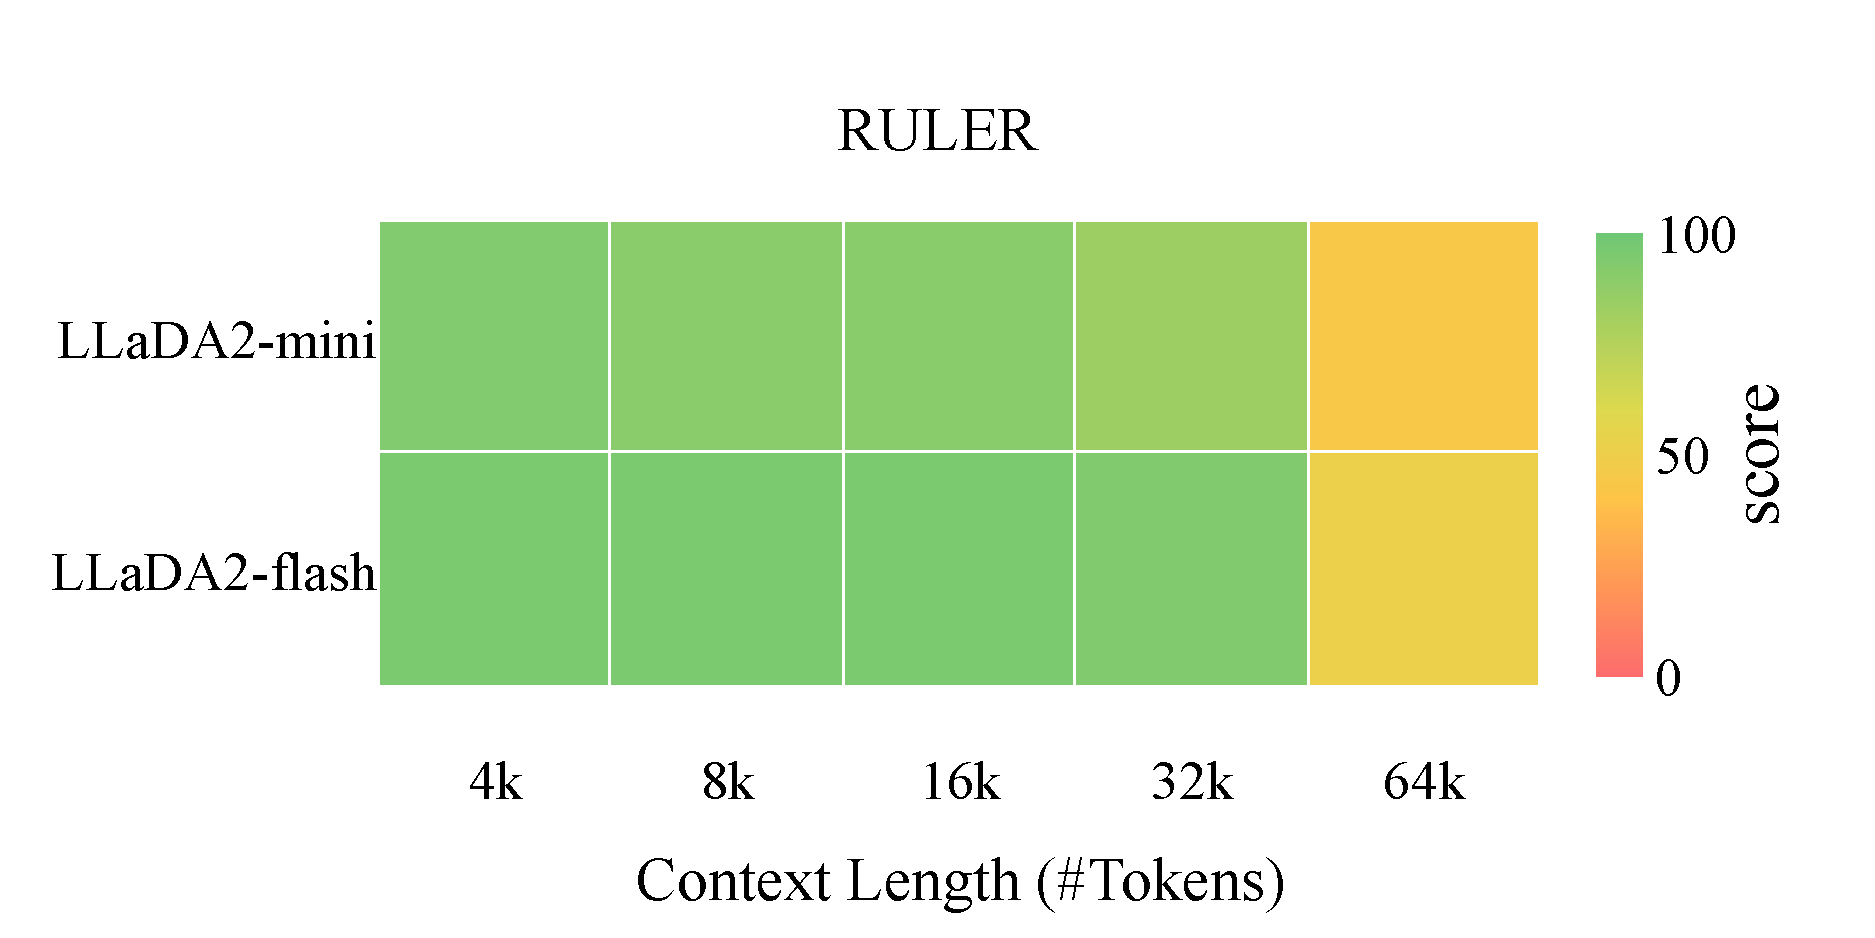
\includegraphics[width=\linewidth]{images/ctxlen.pdf}
        \caption{Performance on the RULER benchmark.}
        \label{fig:ctxlen}
    \end{minipage}
    \vspace{-2ex}
\end{figure}

\textbf{Denoising Threshold}. We first investigate the impact of the Denoising Threshold. While keeping the Block Size fixed at 32, we varied the threshold and observed its effect on quality and speed. As shown in \Cref{fig:params}, the results reveal a clear trade-off. A threshold of 0.95 achieved the highest quality score (70.15) at the cost of the lowest inference speed (2.55 TPF). Lowering the threshold to 0.85 boosted the speed to its peak (3.31 TPF), but led to an unacceptable degradation in quality, with the score dropping to 67.90.

\textbf{Block Size}. Subsequently, we analyze the effect of Block Size. We set the Denoising Threshold to 0.95, the optimal value identified in the prior experiment. The results in \Cref{fig:params} demonstrate a similar trade-off. A block size of 16 yielded the highest score (70.26) but with the slowest inference (2.44 TPF). In contrast, increasing the block size to 32 substantially improved the speed to 2.55 TPF with only a marginal quality drop to 70.15. Further increasing the block size to 64 proved suboptimal, as it degraded both score and speed relative to the size-32 setting. Therefore, a block size of 32 emerges as the most compelling choice, offering a significant speed-up for a negligible performance cost.

\textit{In summary}, based on this analysis, the configuration for our main evaluation is well-supported. The Denoising Threshold of 0.95 is the clear choice for maximizing quality. For block-size, the setting of 32 represents an optimal balance, providing the highest throughput with virtually no sacrifice in performance compared to the slightly higher-scoring but slower setting of 16.

\paragraph{Analysis of Context Length}

To rigorously validate our model's performance across various context lengths, we conducted a series of evaluations using the RULER benchmark.

As shown in \Cref{fig:ctxlen}, both models demonstrate strong performance and stability within context length of 32k. The LLaDA2.0-flash model is particularly robust, maintaining a score above 93 across all lengths from 4k to 32k. The LLaDA2.0-mini model also achieves high scores, starting at 93.29 for 4k but showing a degradation to 83.94 at 32k.

To test the models' extrapolation capabilities, we extended the context length to 64k. This was achieved by employing dynamic RoPE scaling during inference, specifically using the YaRN method with a scaling factor of 2.0. However, this extension resulted in a performance degradation for both models, demonstrating a clear trade-off between context length extension and task accuracy.

\textit{In summary}, this evaluation highlights two key findings: (1) The LLaDA2.0 models are exceptionally robust for long-context tasks within their native 32k window. (2) They can be successfully extended to handle 64k sequences via YaRN scaling, providing flexibility for extreme-length applications, albeit with a predictable performance cost.